\documentclass[a4paper,11pt]{beamer}
\usepackage{etex}
\usepackage{lmodern}
\usepackage[french]{babel}
\usepackage[T1]{fontenc}
\usepackage[utf8]{inputenc}
% \usepackage{listings}
\usepackage{graphicx} 
\usepackage{ragged2e}  
% \usepackage{array}
% \usepackage{tikz} 
% \usepackage{pgf-umlcd} 
\usepackage{csquotes}
\usepackage[pdf]{pstricks}
\usepackage{pst-sigsys}
\usepackage{amsmath,amsfonts,bm}
\usepackage{pstricks-add}
% \usepackage{physics}
% \usepackage{ulem}
% \usepackage{wasysym}
% \usepackage{hyperref}
% \usepackage{color}

\setbeamertemplate{navigation symbols}{}  
  
\usetheme{Darmstadt} 
\setbeamertemplate{footline}{\insertframenumber/\inserttotalframenumber}
\title{L3 - CMI017 : Signaux et Systèmes\\Séquence I}
\author{BULOUP Frank}
\institute{Aix Marseille Université\\Institut des Sciences du Mouvement}
\date{}

\setbeamertemplate{footline} 
{  
	\begin{beamercolorbox}[ht=2.5ex,dp=1.125ex,%
      leftskip=.3cm,rightskip=.3cm plus1fil]{title in head/foot}%
      {\usebeamerfont{title in head/foot}\insertshorttitle} \hfill    
      \insertframenumber / \inserttotalframenumber%
    \end{beamercolorbox}%
%     \begin{beamercolorbox}[colsep=1.5pt]{lower separation line foot}
%     \end{beamercolorbox} 
}

\newcounter{exampleBlockCounter}
\setcounter{exampleBlockCounter}{1}

\definecolor{comment}{rgb}{0.12, 0.38, 0.18 } %adjusted, in Eclipse: {0.25, 0.42, 0.30 } = #3F6A4D
\definecolor{keyword}{rgb}{0.37, 0.08, 0.25}  % #5F1441
\definecolor{string}{rgb}{0.06, 0.10, 0.98} % #101AF9
\definecolor{myGreen}{rgb}{0,0.4,0}

% \lstset {language=Java,
%  frame=single,
%  frameround=tttt,
%  rulesepcolor=\color{black},
%  showspaces=false,showtabs=false,tabsize=2,
%  numberstyle=\tiny,numbers=left,
%  stringstyle=\color{string},
%  keywordstyle = \color{keyword}\bfseries,
%  commentstyle=\color{comment}\itshape,
%  basicstyle=\ttfamily\footnotesize,
%  breaklines=true,
%  captionpos=b
% }

% \renewenvironment{package}[2][\umlcdPackageTitle]{
% \edef\umlcdPackageTitle{#2}
% \def\umlcdPackageFit{}
% \def\umlcdPackageName{#1}
% }{
%   \begin{pgfonlayer}{background}
%   \node[umlcd style, draw, inner sep=0.5cm, fit = \umlcdPackageFit] (\umlcdPackageName) {};
%   \node[umlcd style, draw, outer ysep=-0.5, anchor=south west] (\umlcdPackageName caption) at
%   (\umlcdPackageName.north west) {\umlcdPackageTitle};
%   \end{pgfonlayer}
% }

\begin{document}

\begin{frame}[plain]  
	\titlepage 
	\center{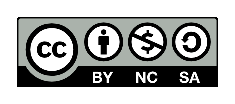
\includegraphics[scale=0.75]{images/by-nc-sa.eps}}
	\vspace{1cm}
	
	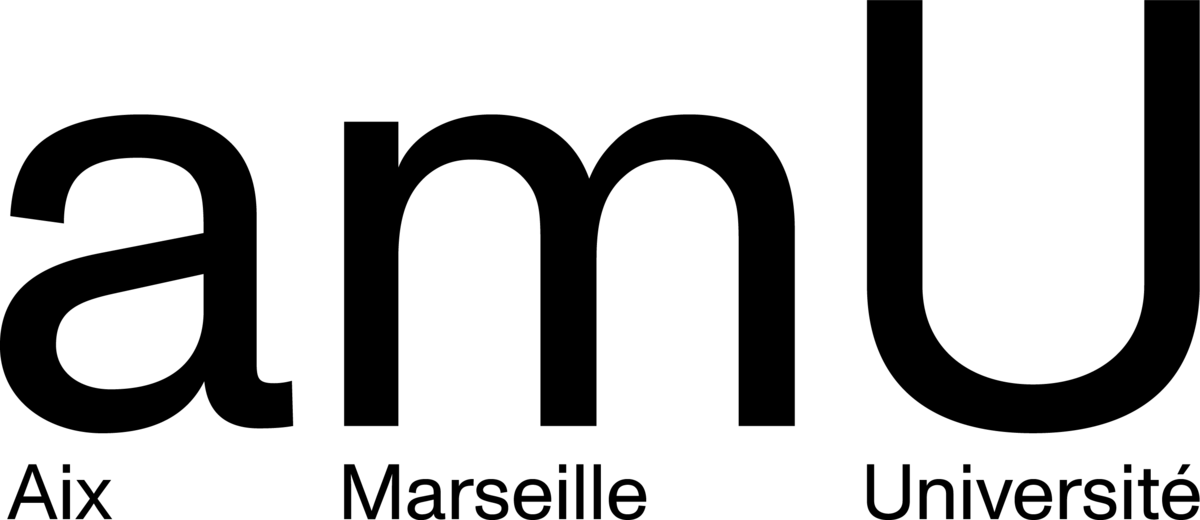
\includegraphics[scale=0.6]{images/LogoAMU.png}\hspace*{2cm}
	
\includegraphics[scale=0.2]{images/LogoCNRS.eps}\hspace*{2cm}
	
\includegraphics[scale=0.1]{images/LogoISM.eps}
\end{frame} 
 
 
\begin{frame}{Plan de cette séquence}
	\tableofcontents[hideallsubsections]
\end{frame}

\AtBeginSection[]{
\begin{frame}{Signaux et Systèmes}
	\tableofcontents[currentsection,hideallsubsections]
\end{frame}
}

\section{Concepts de Signaux continu et discret}
\subsection{Signal continu} 
\begin{frame}
\centering
Savez-vous ce qu'est un \textbf{signal continu} ?

\pause
\vspace{1cm}
\huge $\Leftrightarrow$ 

\small
\vspace{1cm} 
\begin{itemize}
  \item Qu'est-ce qu'un \textbf{signal} ?
  \item Dans quel cas un signal est qualifié de \textbf{continu} ?
\end{itemize}
\end{frame}

\begin{frame}
\centering
Voici quelques exemples pour vous aider :
\vspace{1cm}

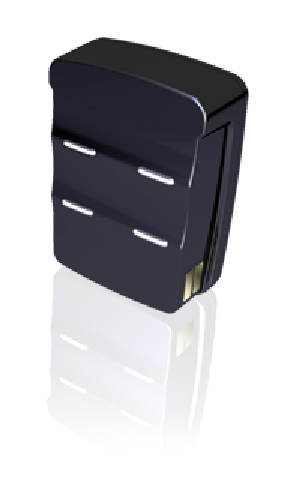
\includegraphics[scale=.5]{images/EMG.eps}\hspace*{2cm}
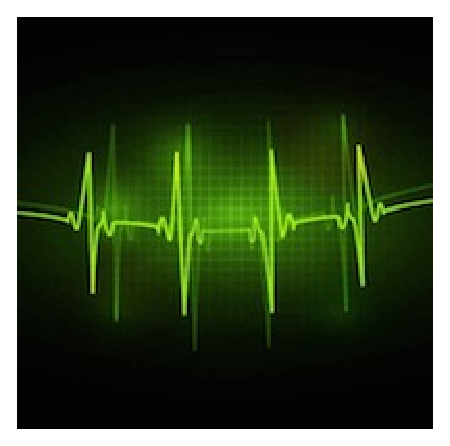
\includegraphics[scale=.25]{images/ECG.eps}\hspace*{2cm}
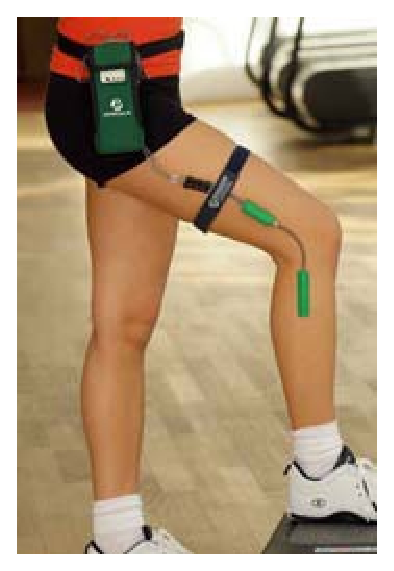
\includegraphics[scale=.25]{images/Gonio.eps}
\end{frame}

\begin{frame}
\begin{block}{Définition du terme \enquote{\textbf{signal}}}
\justifying
Dans le domaine de l'ingéniérie électrique, un signal est une manifestation d'un
phénomène physique observable électriquement.
\end{block}
\pause
\begin{block}{Définition du terme \enquote{\textbf{continu}}}
\justifying
La notion de continu signifie que la grandeur électrique associée à ce signal
peut prendre n'importe quelle valeur dans un intervalle donné de valeurs réelles.
\end{block}
\vspace{1cm}
\centering
\textbf{\textcolor{red}{$\Leftrightarrow$ Lié à la notion de capteur}}
\end{frame}

\begin{frame}
\centering
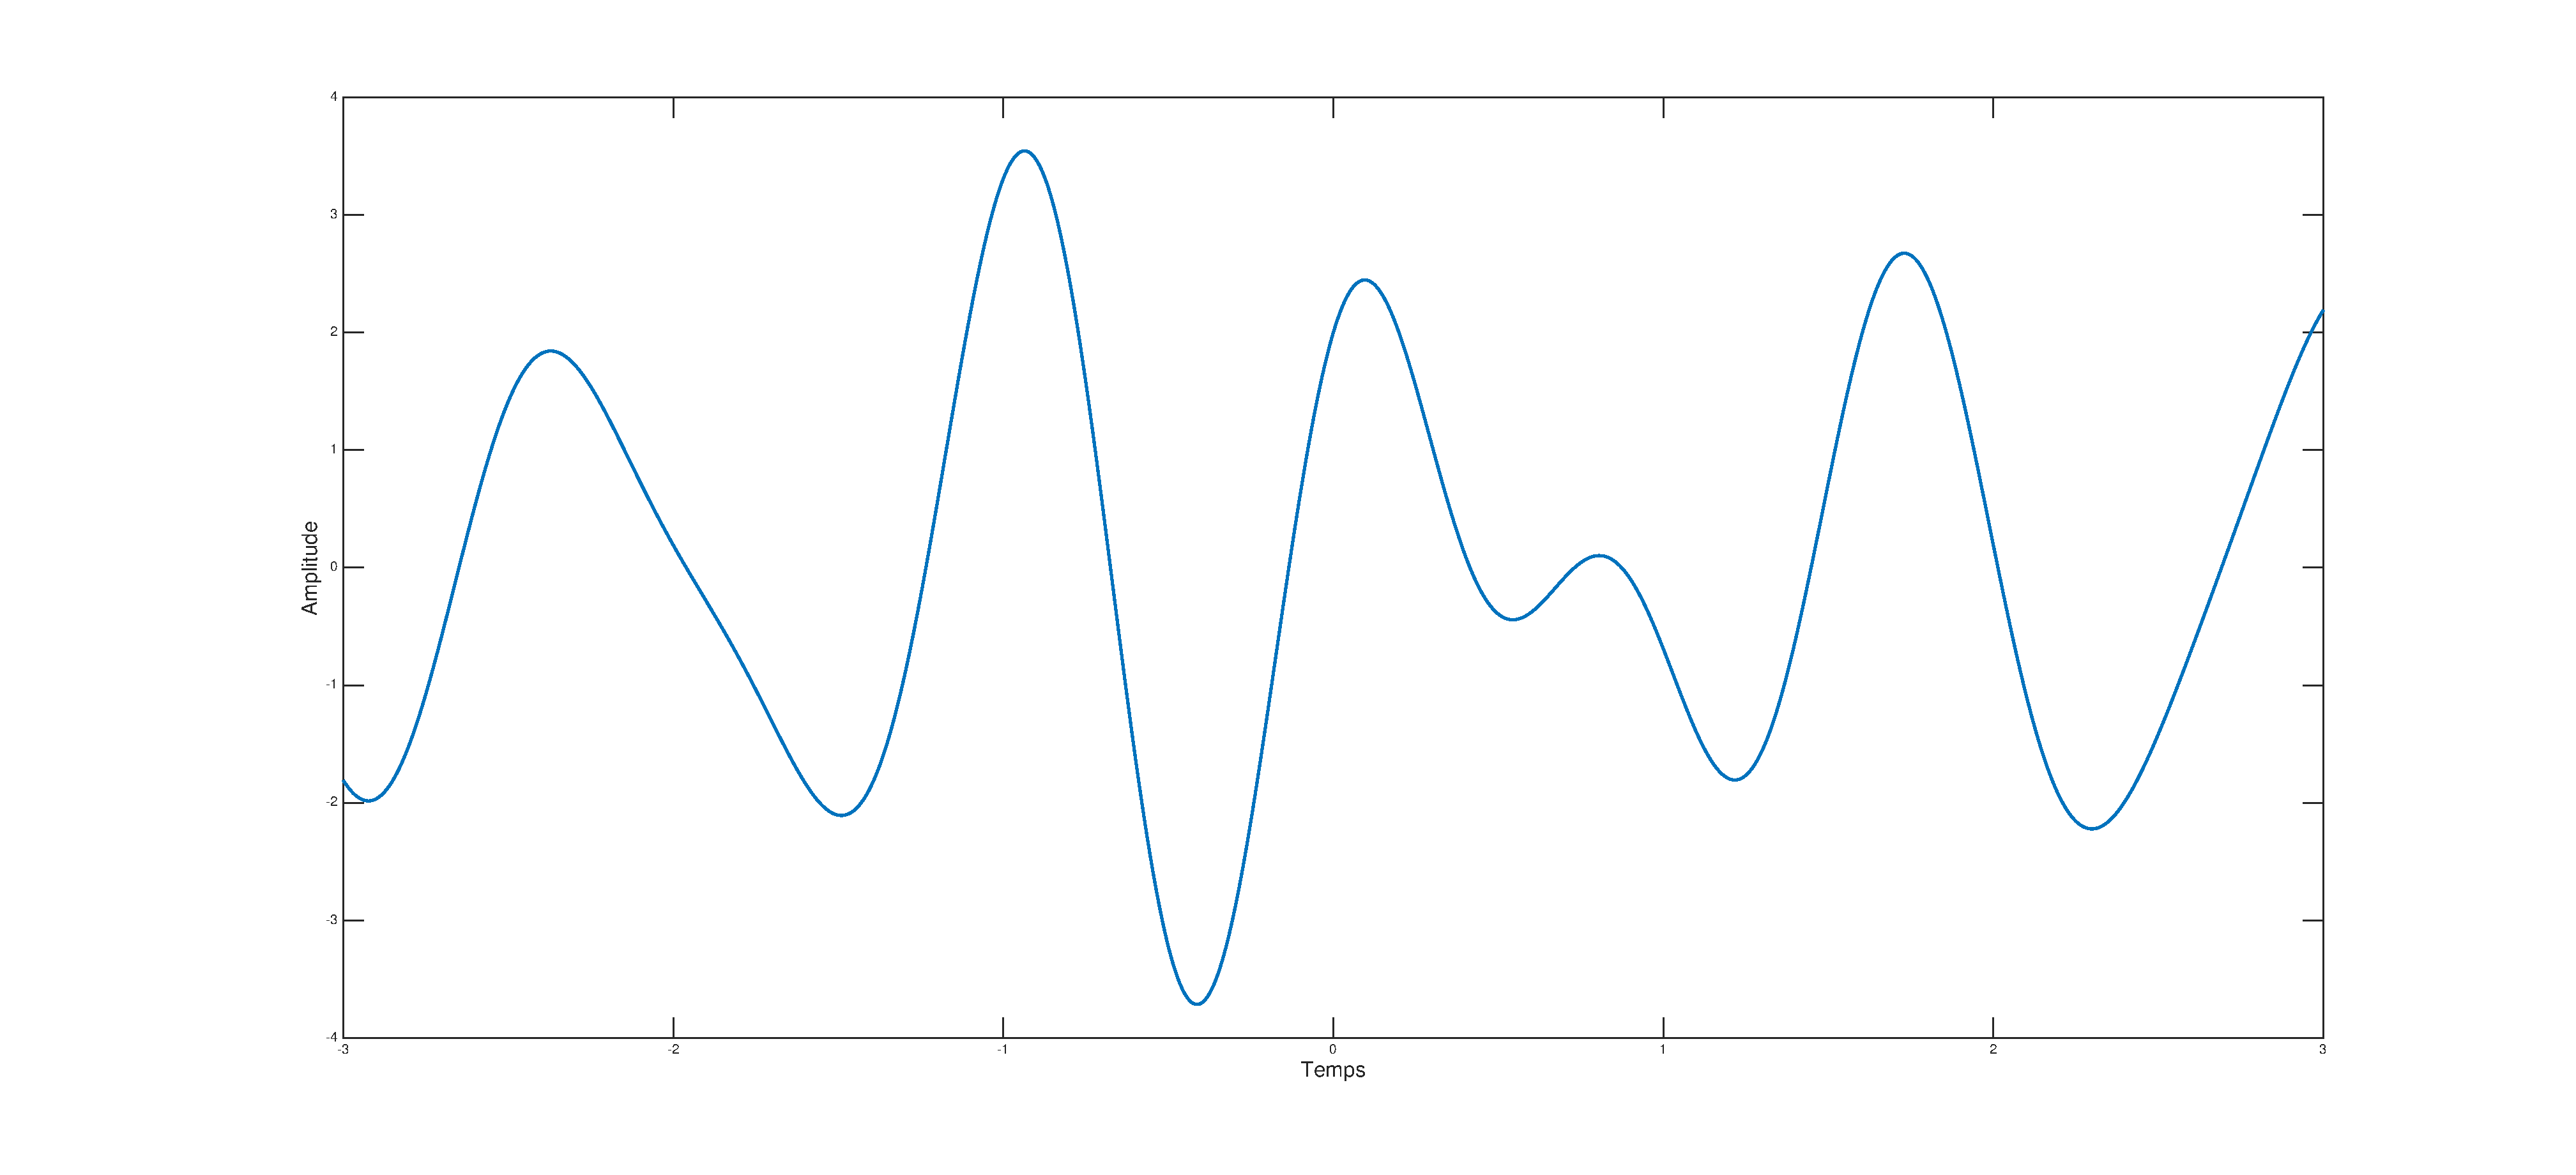
\includegraphics[scale=.15]{images/GenSinus.eps}
$$
s(t) = cos(2\pi1t) + cos(2\pi1.2t) + 2sin(2\pi0.75t)
$$
\end{frame}

\subsection{Signal discret} 
\begin{frame}
\centering
Par opposition à \enquote{\textbf{continu}} !
\vspace{0.5cm}

\centering

\includegraphics[scale=.15]{images/audio.eps}\hspace*{2cm}

\includegraphics[scale=.15]{images/video.eps}\\

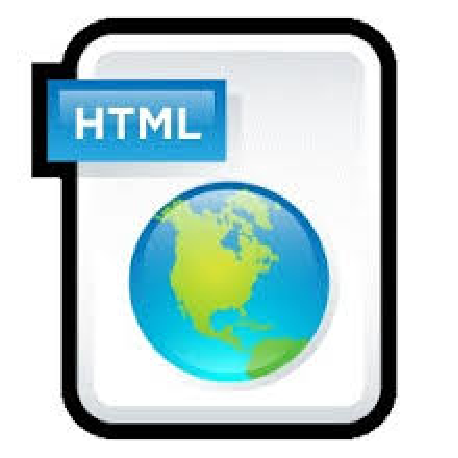
\includegraphics[scale=.15]{images/web.eps}

\pause
\vspace{0.5cm}
\justifying
De façon générale, tout fichier, toute donnée ayant été enregistrée sur un
dispositif numérique
\begin{itemize}
  \item ordinateur
  \item tablette
  \item téléphone portable
  \item \ldots
\end{itemize}
\end{frame}

\begin{frame}
\begin{exampleblock}{Exercice \Roman{exampleBlockCounter}}
Tracer le signal suivant en utilisant Matlab :
$$
s(t) = cos(2\pi1t) + cos(2\pi1.2t) + 2sin(2\pi0.75t)
$$
\begin{enumerate}
  \item Créer le vecteur temporel discret correspondant (pas de $\frac{1}{10}$
  de seconde)
  \item Tracer le signal en utilisant la commande \textbf{plot}
  \item Mettre en évidence la discrétisation en éditant le graphe
  \item Tracer le signal en utilisant la commande \textbf{stem}
\end{enumerate}
\end{exampleblock}
\pause
\centering
\textcolor{red}{\textbf{Plusieurs versions discrètes d'un signal sont possibles
: cela dépend de la résolution temporelle (notion d'échantillonnage)}}
\end{frame}
\stepcounter{exampleBlockCounter}

\begin{frame}
\centering
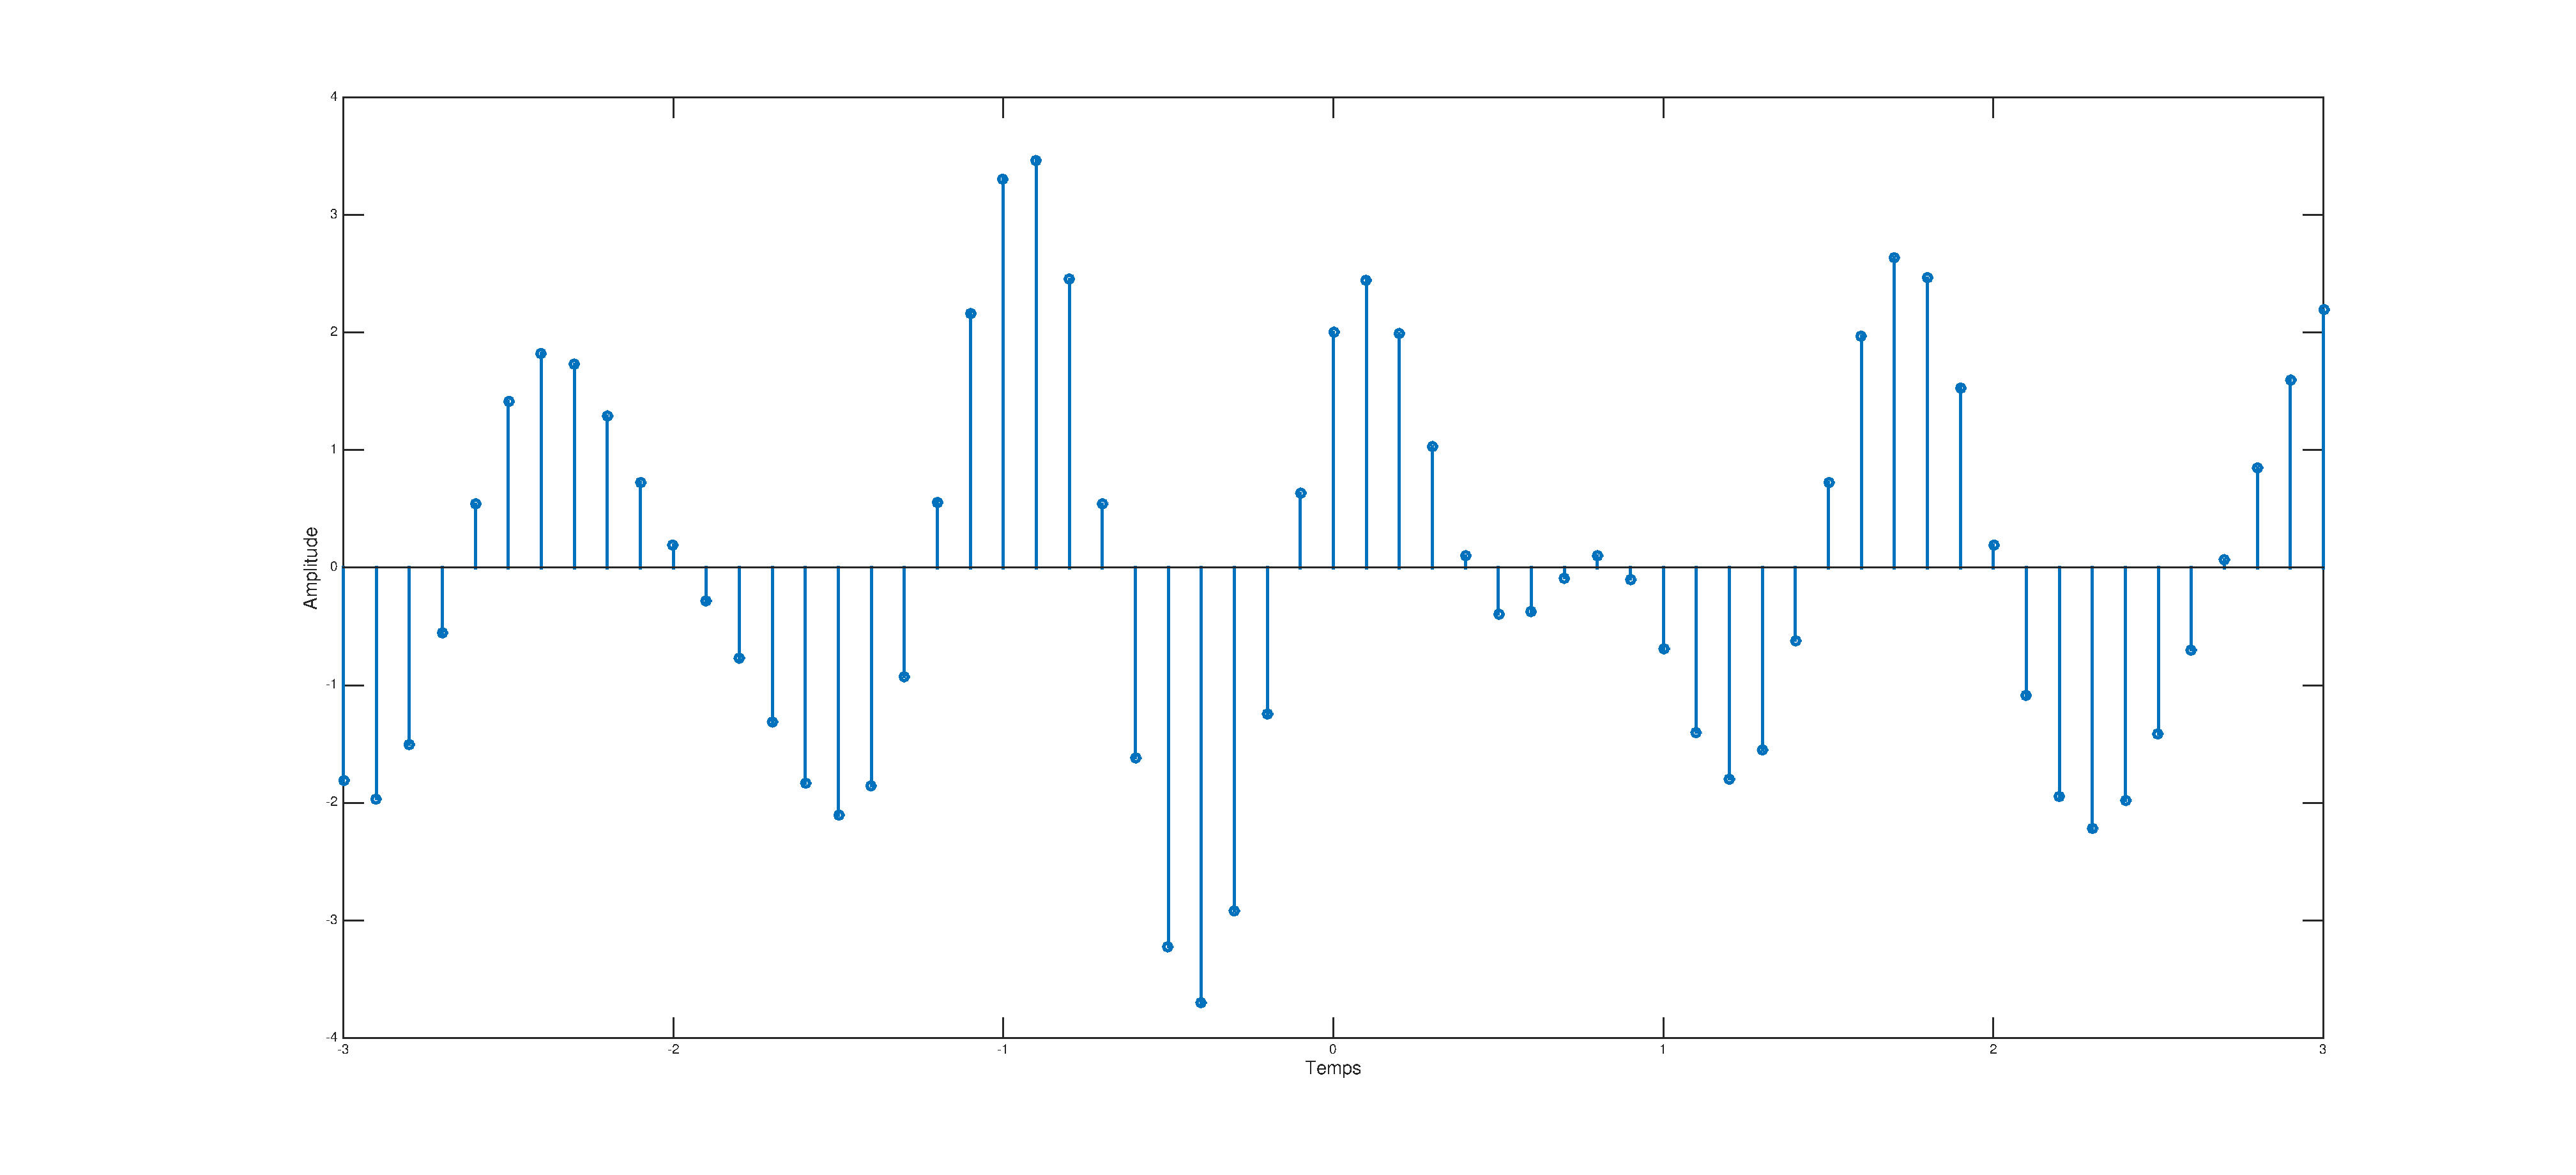
\includegraphics[scale=.125]{images/GenSinusDiscret.eps}
$$
\begin{aligned}
s(n\Delta t) &= cos(2\pi1n\Delta t) + cos(2\pi1.2n\Delta t) +
2sin(2\pi0.75n\Delta t)\\
s(n) &= cos(2\pi1n\Delta t) + cos(2\pi1.2n\Delta t) +
2sin(2\pi0.75n\Delta t)
\end{aligned}
$$
\end{frame}


\section{Concepts de Systèmes continu et discret}
\subsection{Système continu} 
\begin{frame}

\begin{figure}
	\begin{pspicture}[showgrid=false](0,0)(9,2)
		\psset{arrows=->}
%		\pssignal(1.5,1){e}{
%		$\begin{cases}
%		\text{Signal d'entrée}\\
%		e(t)
%		\end{cases}$
%		}
%		\psfblock[framesize=1.75 1.65](4.5,1){h}{Système}
%		\ncline{e}{h}
%		\pssignal(7.5,1){s}{$\begin{cases}
%		\text{Signal de sortie}\\
%		s(t)
%		\end{cases}$}
%		\ncline{h}{s}
	\end{pspicture}
\end{figure}
\begin{block}{Définition}
\centering
Un système continu est un dispositif qui transforme un signal continu
\end{block}
\begin{itemize}
\justifying
  \item Il est caractérisé par une équation différentielle (ED)
  \item La transformation dépend du type et des valeurs des paramètres de cette équation
\end{itemize}
\end{frame}

\begin{frame}
\justifying
Voici quelques exemples d'équations différentielles :
\begin{align}
  s' &= \bm{\textcolor{blue}{\gamma}} e\\
  s''+ \bm{\textcolor{blue}{\mu}} s' &= \bm{\textcolor{blue}{\gamma}}
  e\\
  \bm{\textcolor{blue}{t}} \cdot s' &= \bm{\textcolor{blue}{\gamma}} e\\
  (s')^{\bm{\textcolor{blue}{2}}} &= \bm{\textcolor{blue}{\gamma}} e
\end{align}
\centering
\textcolor{blue}{\textbf{Les caractères en bleu sont les paramètres}}
\end{frame}

\begin{frame}
\justifying
Voici quelques exemples d'équations différentielles :
\setcounter{equation}{0}
\begin{align}
  s' &= \bm{\textcolor{blue}{\gamma}} e\\
  s''+ \bm{\textcolor{blue}{\mu}} s' &= \bm{\textcolor{blue}{\gamma}}
  e\\
  \bm{\textcolor{blue}{t}} \cdot s' &= \bm{\textcolor{blue}{\gamma}} e\\
  (s')^{\bm{\textcolor{blue}{2}}} &= \bm{\textcolor{blue}{\gamma}} e
\end{align}
\centering
\textcolor{blue}{\textbf{$\Rightarrow$ Si ces paramètres sont constants dans le
temps, le système est dit invariant}}
\vspace{1cm}

\pause
\textcolor{myGreen}{\textbf{Parmi les équation précédentes, quelles sont celles
qui caractérisent un système invariant ?}}
\end{frame}

\begin{frame}
\justifying
Voici quelques exemples d'équations différentielles :
\setcounter{equation}{0}
\begin{align}
  s' &= \bm{\textcolor{blue}{\gamma}} e \textcolor{myGreen}{\:\checkmark}\\
  s''+ \bm{\textcolor{blue}{\mu}} s' &= \bm{\textcolor{blue}{\gamma}}
  e \textcolor{myGreen}{\:\checkmark}\\
  \bm{\textcolor{blue}{t}} \cdot s' &= \bm{\textcolor{blue}{\gamma}} e\\
  (s')^{\bm{\textcolor{blue}{2}}} &= \bm{\textcolor{blue}{\gamma}} e \textcolor{myGreen}{\:\checkmark}
\end{align}
\centering
\textcolor{blue}{\textbf{$\Rightarrow$ Si ces paramètres sont constants dans le
temps, le système est dit invariant}}
\vspace{1cm}

\textcolor{myGreen}{\textbf{Parmi les équation précédentes, quelles sont celles
qui caractérisent un système invariant ?}}
\end{frame}

\begin{frame}
\begin{block}{Invariance temporelle (Stationnarité)}
Étant donné :
\begin{figure}
	\begin{pspicture}[showgrid=false](0,0)(9,0.5)
		\psset{arrows=->}
		\pssignal(1.5,0.25){e1}{$e(t)$}
		\psfblock[framesize=1.75 0.65](4.5,0.25){h1}{Système}
		\ncline{e1}{h1}
		\pssignal(7.5,0.25){s1}{$s(t)$}
		\ncline{h1}{s1}
	\end{pspicture}
\end{figure}
le système est invariant si : 
\begin{figure}
	\begin{pspicture}[showgrid=false](0,0)(9,0.5)
		\psset{arrows=->}
		\pssignal(1.5,0.25){e2}{$e(t - \tau)$}
		\psfblock[framesize=1.75 0.65](4.5,0.25){h2}{Système}
		\ncline{e2}{h2}
		\pssignal(7.5,0.25){s2}{$s(t - \tau)$}
		\ncline{h2}{s2}
	\end{pspicture}
\end{figure}
\end{block}
\end{frame}

\begin{frame}
\begin{block}{Linéarité}
Étant donné :
\begin{figure}
	\begin{pspicture}[showgrid=false](0,0)(9,0.5)
		\psset{arrows=->}
		\pssignal(1.5,0.25){e1}{$e_{1}(t)$}
		\psfblock[framesize=1.75 0.65](4.5,0.25){h1}{Système}
		\ncline{e1}{h1}
		\pssignal(7.5,0.25){s1}{$s_{1}(t)$}
		\ncline{h1}{s1}
	\end{pspicture}
\end{figure}
et : 
\begin{figure}
	\begin{pspicture}[showgrid=false](0,0)(9,0.5)
		\psset{arrows=->}
		\pssignal(1.5,0.25){e2}{$e_{2}(t)$}
		\psfblock[framesize=1.75 0.65](4.5,0.25){h2}{Système}
		\ncline{e2}{h2}
		\pssignal(7.5,0.25){s2}{$s_{2}(t)$}
		\ncline{h2}{s2}
	\end{pspicture}
\end{figure}
le système est linéaire si :
\begin{figure}
	\begin{pspicture}[showgrid=false](0,0)(9,0.5)
		\psset{arrows=->}
		\pssignal(1.5,0.25){e}{$\alpha e_{1}(t) + \beta e_{2}(t)$}
		\psfblock[framesize=1.75 0.65](4.5,0.25){h}{Système}
		\ncline{e}{h}
		\pssignal(7.5,0.25){s}{$\alpha s_{1}(t) + \beta s_{2}(t)$}
		\ncline{h}{s}
	\end{pspicture}
\end{figure}
est vrai pour tout $\alpha$ et $\beta$
\end{block}
\end{frame}

\begin{frame}
\justifying
Voici quelques exemples d'équations différentielles :
\setcounter{equation}{0}
\begin{align}
  s' &= \bm{\textcolor{blue}{\gamma}} e\\
  s''+ \bm{\textcolor{blue}{\mu}} s' &= \bm{\textcolor{blue}{\gamma}} e\\
  \bm{\textcolor{blue}{t}} \cdot s' &= \bm{\textcolor{blue}{\gamma}} e\\
  (s')^{\bm{\textcolor{blue}{2}}} &= \bm{\textcolor{blue}{\gamma}} e
\end{align}
\centering

\textcolor{myGreen}{\textbf{Parmi les équations précédentes, quelles sont celles
qui caractérisent un système linéaire ?}}
\end{frame}

\begin{frame}
\justifying
Voici quelques exemples d'équations différentielles :
\setcounter{equation}{0}
\begin{align}
  s' &= \bm{\textcolor{blue}{\gamma}} e \textcolor{myGreen}{\:\checkmark}\\
  s''+ \bm{\textcolor{blue}{\mu}} s' &= \bm{\textcolor{blue}{\gamma}}
  e \textcolor{myGreen}{\:\checkmark}\\
  \bm{\textcolor{blue}{t}} \cdot s' &= \bm{\textcolor{blue}{\gamma}}
  e\textcolor{myGreen}{\:\checkmark}\\
  (s')^{\bm{\textcolor{blue}{2}}} &= \bm{\textcolor{blue}{\gamma}} e 
\end{align}
\centering

\textcolor{myGreen}{\textbf{Parmi les équations précédentes, quelles sont celles
qui caractérisent un système linéaire ?}}
\end{frame}

\begin{frame}
\begin{alertblock}{Linéarité et Invariance Temporelle}
\center
Système Continu Linéaire et Invariant dans le Temps (SCLIT) 
\end{alertblock}
\begin{exampleblock}{Exercice \Roman{exampleBlockCounter}}
\justifying
Quelles sont parmi les ED suivantes celles qui caractérisent des SCLIT ?
\setcounter{equation}{0}
\begin{align}
  s' - 2 \cdot s &= e \\
  s' + t \cdot s &= e \\
  s'' + s^2 &= e 
\end{align}
\end{exampleblock}
\end{frame}

\begin{frame}
\begin{alertblock}{Linéarité et Invariance Temporelle}
\center
Système Continu Linéaire et Invariant dans le Temps (SCLIT) 
\end{alertblock}
\begin{exampleblock}{Exercice \Roman{exampleBlockCounter}}
\justifying
Quelles sont parmi les ED suivantes celles qui caractérisent des SCLIT ?
\setcounter{equation}{0}
\begin{align}
  s' - 2 \cdot s &= e \textcolor{myGreen}{\:\checkmark}\\
  s' + t \cdot s &= e\\
  s'' + s^2 &= e
\end{align}
\end{exampleblock}
\stepcounter{exampleBlockCounter}
\end{frame}

\subsection{Système discret : mêmes démarches !} 

\begin{frame}

\begin{figure}
	\begin{pspicture}[showgrid=false](0,0)(9,2)
		\psset{arrows=->}
		\pssignal(1.5,1){e}{$\begin{cases}
		\text{Signal d'entrée}\\
		e(nTe)\\
		e(n)
		\end{cases}$}
		\psfblock[framesize=1.75 1.65](4.5,1){h}{Système}
		\ncline{e}{h}
		\pssignal(7.5,1){s}{$\begin{cases}
		\text{Signal de sortie}\\
		s(nTe)\\
		s(n)
		\end{cases}$}
		\ncline{h}{s}
	\end{pspicture}
\end{figure}
\begin{block}{Définition}
\centering
Un système discret est un algorithme qui transforme un signal discret
\end{block}
\begin{itemize}
\justifying
  \item Il est caractérisé par une équation aux différences (EAD)
  \item La transformation dépend du type et des valeurs des paramètres de
  cette équation
\end{itemize}
\end{frame}


\begin{frame}
\justifying
Voici quelques exemples d'équations aux différences :
\setcounter{equation}{0}
\begin{align}
  s(n) &= \bm{\textcolor{blue}{\gamma}} e(n)\\
  s(n-2) + \bm{\textcolor{blue}{\mu}} s(n-1) &= \bm{\textcolor{blue}{\gamma}}
  e(n)\\
  \bm{\textcolor{blue}n} \cdot s(n) &= \bm{\textcolor{blue}{\gamma}} e(n)\\
  (s(n))^{\bm{\textcolor{blue}{2}}} &= \bm{\textcolor{blue}{\gamma}} e(n)
\end{align}
\centering
\textcolor{blue}{\textbf{Les caractères en bleu sont les paramètres}}
\end{frame}

\begin{frame}
\justifying
Voici quelques exemples d'équations aux différences :
\setcounter{equation}{0}
\begin{align}
  s(n) &= \bm{\textcolor{blue}{\gamma}} e(n)\\
  s(n-2) + \bm{\textcolor{blue}{\mu}} s(n-1) &= \bm{\textcolor{blue}{\gamma}}
  e(n)\\
  \bm{\textcolor{blue}n} \cdot s(n) &= \bm{\textcolor{blue}{\gamma}} e(n)\\
  (s(n))^{\bm{\textcolor{blue}{2}}} &= \bm{\textcolor{blue}{\gamma}} e(n)
\end{align}
\centering
\textcolor{blue}{\textbf{$\Rightarrow$ Si ces paramètres sont constants dans le
temps, le système est dit invariant}}
\vspace{1cm}

\pause
\textcolor{myGreen}{\textbf{Parmi les équations précédentes, quelles sont celles
qui caractérisent un système invariant ?}}
\end{frame}

\begin{frame}
\justifying
Voici quelques exemples d'équations aux différences :
\setcounter{equation}{0}
\begin{align}
  s(n) &= \bm{\textcolor{blue}{\gamma}} e(n)\textcolor{myGreen}{\:\checkmark}\\
  s(n-2) + \bm{\textcolor{blue}{\mu}} s(n-1) &= \bm{\textcolor{blue}{\gamma}}
  e(n)\textcolor{myGreen}{\:\checkmark}\\
  \bm{\textcolor{blue}n} \cdot s(n) &= \bm{\textcolor{blue}{\gamma}} e(n)\\
  (s(n))^{\bm{\textcolor{blue}{2}}} &= \bm{\textcolor{blue}{\gamma}} e(n)\textcolor{myGreen}{\:\checkmark}
\end{align}
\centering
\textcolor{blue}{\textbf{$\Rightarrow$ Si ces paramètres sont constants dans le
temps, le système est dit invariant}}
\vspace{1cm}

\textcolor{myGreen}{\textbf{Parmi les équations précédentes, quelles sont celles
qui caractérisent un système invariant ?}}
\end{frame}

\begin{frame}
\begin{block}{Invariance temporelle (Stationnarité)}
Étant donné :
\begin{figure}
	\begin{pspicture}[showgrid=false](0,0)(9,0.5)
		\psset{arrows=->}
		\pssignal(1.5,0.25){e1}{$e(n)$}
		\psfblock[framesize=1.75 0.65](4.5,0.25){h1}{Système}
		\ncline{e1}{h1}
		\pssignal(7.5,0.25){s1}{$s(n)$}
		\ncline{h1}{s1}
	\end{pspicture}
\end{figure}
le système est invariant si : 
\begin{figure}
	\begin{pspicture}[showgrid=false](0,0)(9,0.5)
		\psset{arrows=->}
		\pssignal(1.5,0.25){e2}{$e(n - n_0)$}
		\psfblock[framesize=1.75 0.65](4.5,0.25){h2}{Système}
		\ncline{e2}{h2}
		\pssignal(7.5,0.25){s2}{$s(n - n_0)$}
		\ncline{h2}{s2}
	\end{pspicture}
\end{figure}
\end{block}
\end{frame}

\begin{frame}
\begin{block}{Linéarité}
Étant donné :
\begin{figure}
	\begin{pspicture}[showgrid=false](0,0)(9,0.5)
		\psset{arrows=->}
		\pssignal(1.5,0.25){e1}{$e_{1}(n)$}
		\psfblock[framesize=1.75 0.65](4.5,0.25){h1}{Système}
		\ncline{e1}{h1}
		\pssignal(7.5,0.25){s1}{$s_{1}(n)$}
		\ncline{h1}{s1}
	\end{pspicture}
\end{figure}
et : 
\begin{figure}
	\begin{pspicture}[showgrid=false](0,0)(9,0.5)
		\psset{arrows=->}
		\pssignal(1.5,0.25){e2}{$e_{2}(n)$}
		\psfblock[framesize=1.75 0.65](4.5,0.25){h2}{Système}
		\ncline{e2}{h2}
		\pssignal(7.5,0.25){s2}{$s_{2}(n)$}
		\ncline{h2}{s2}
	\end{pspicture}
\end{figure}
le système est linéaire si :
\begin{figure}
	\begin{pspicture}[showgrid=false](0,0)(9,0.5)
		\psset{arrows=->}
		\pssignal(1.5,0.25){e}{$\alpha e_{1}(n) + \beta e_{2}(n)$}
		\psfblock[framesize=1.75 0.65](4.5,0.25){h}{Système}
		\ncline{e}{h}
		\pssignal(7.5,0.25){s}{$\alpha s_{1}(n) + \beta s_{2}(n)$}
		\ncline{h}{s}
	\end{pspicture}
\end{figure}
est vrai pour tout $\alpha$ et $\beta$
\end{block}
\end{frame}

\begin{frame}
\justifying
Voici quelques exemples d'équations aux différences :
\setcounter{equation}{0}
\begin{align}
  s(n) &= \bm{\textcolor{blue}{\gamma}} e(n)\\
  s(n-2) + \bm{\textcolor{blue}{\mu}} s(n-1) &= \bm{\textcolor{blue}{\gamma}}
  e(n)\\
  \bm{\textcolor{blue}n} \cdot s(n) &= \bm{\textcolor{blue}{\gamma}} e(n)\\
  (s(n))^{\bm{\textcolor{blue}{2}}} &= \bm{\textcolor{blue}{\gamma}} e(n)
\end{align}
\centering

\textcolor{myGreen}{\textbf{Parmi les équations précédentes, quelles sont celles
qui caractérisent un système linéaire ?}}
\end{frame}

\begin{frame}
\justifying
Voici quelques exemples d'équations aux différences :
\setcounter{equation}{0}
\begin{align}
  s(n) &= \bm{\textcolor{blue}{\gamma}} e(n)\textcolor{myGreen}{\:\checkmark}\\
  s(n-2) + \bm{\textcolor{blue}{\mu}} s(n-1) &= \bm{\textcolor{blue}{\gamma}}
  e(n)\textcolor{myGreen}{\:\checkmark}\\
  \bm{\textcolor{blue}n} \cdot s(n) &= \bm{\textcolor{blue}{\gamma}}
  e(n)\textcolor{myGreen}{\:\checkmark}\\
  (s(n))^{\bm{\textcolor{blue}{2}}} &= \bm{\textcolor{blue}{\gamma}} e(n)
\end{align}
\centering

\textcolor{myGreen}{\textbf{Parmi les équations précédentes, quelles sont celles
qui caractérisent un système linéaire ?}}
\end{frame}

\begin{frame}
\begin{alertblock}{Linéarité et Invariance Temporelle}
\center
Système Discret Linéaire et Invariant dans le Temps (SDLIT) 
\end{alertblock}
\begin{exampleblock}{Exercice \Roman{exampleBlockCounter}}
\justifying
Quelles sont parmi les EAD suivantes celles qui caractérisent des SDLIT ?
\setcounter{equation}{0}
\begin{align}
  s(n) &= \frac{e(n)-e(n-1)}{T}\\
  2s(n+1) - s(n)  &= \frac{e(n)}{s(n)}\\
  s(n+1) + n\cdot s(n) &= e(n)
\end{align}
\end{exampleblock}
\end{frame}

\begin{frame}
\begin{alertblock}{Linéarité et Invariance Temporelle}
\center
Système Discret Linéaire et Invariant dans le Temps (SDLIT) 
\end{alertblock}
\begin{exampleblock}{Exercice \Roman{exampleBlockCounter}}
\justifying
Quelles sont parmi les EAD suivantes celles qui caractérisent des SDLIT ?
\setcounter{equation}{0}
\begin{align}
  s(n) &= \frac{e(n)-e(n-1)}{T}\textcolor{myGreen}{\:\checkmark}\\
  2s(n+1) - s(n) &= \frac{e(n)}{s(n)}\\
  s(n+1) + n\cdot s(n) &= e(n)
\end{align}
\end{exampleblock}
\stepcounter{exampleBlockCounter}
\end{frame}

\section{Représentations des SDLIT}
\begin{frame}
\centering Sur un exemple d'un système nommé $S_1$, on connait déjà :
\vspace{1cm}
\begin{block}{La description textuelle de $S_1$}
\center{Le système calcule une moyenne mobile sur deux échantillons}
\end{block}
\pause
\vspace{1cm}
\begin{block}{L'équation aux différences de $S_1$}
\[
s(n) = \frac{e(n) + e(n-1)}{2}
\]
\end{block}
\end{frame}

\subsection{Diagramme blocs}
\begin{frame}
\begin{block}{Diagramme bloc de $S_1$}
\begin{figure}
	\begin{pspicture}[showgrid=false](0,0)(7,2)
		\psset{arrows=->}
		\pssignal(0.5,1.5){e}{e(n)}
		\pssignal(6.5,1.5){s}{s(n)}
		\psfblock[framesize=1.5 0.75](2.75,0.5){delay}{Retard}
		\pscircleop(4,1.5){add} 
		\pscircleop[operation=times](5,1.5){times}
		\rput(5,1){$\frac{1}{2}$}
		\dotnode(1.5,1.5){node}
		\ncline{e}{add}
		\ncline{add}{times}
		\ncline{times}{s}
		\ncangle[angleA = 0, angleB = -90]{->}{delay}{add}
		\ncangle[angleA = -90, angleB = 180]{->}{node}{delay}
	\end{pspicture}
\end{figure}
\end{block}
\pause
\begin{exampleblock}{Exercice \Roman{exampleBlockCounter}}
Représenter les diagrammes blocs associés à ces EAD :
\setcounter{equation}{0}
\begin{align}
	s(n) &= \frac{e(n)-e(n-1)}{T}\\
	s(n) &= s(n+1)+T\cdot e(n)\\
	s(n) &= e(n) + s(n-1) + s(n-2)
\end{align}
\end{exampleblock}
\stepcounter{exampleBlockCounter}
\end{frame}

\subsection{Notion de réponse impulsionnelle}
\begin{frame}
\begin{block}{Définition de l'impulsion unitaire}
\[
	\delta (n)= 
		\begin{cases}
		1 & \text{si }n=0 \\
		0 & \text{sinon}
		\end{cases}
\]
\end{block}
\begin{alertblock}{Définition}
\centering
La réponse impulsionnelle d'un SDLIT est le signal de sortie de ce système
lorsqu'une impulsion unitaire lui est appliquée en entrée.
\end{alertblock}
\end{frame}

\begin{frame}

\begin{block}{Forme générale de l'EAD}
$$
s(n) = \sum_{k=0}^{N-1}b(k)e(n-k) - \sum_{k=1}^{M-1}a(k)s(n-k)
$$

\begin{itemize}\justifying
  \item $a(k)$ et $b(k)$ sont les paramètres, les coefficients de l'EAD
  \item Matlab possède une fonction nommé \textbf{impz} qui permet de calculer
  directement la réponse impulsionnelle
  \item Ces coefficients peuvent être utilisés directement dans la fonction
  \textbf{impz} de Matlab avec $a(0)=1$
\end{itemize}
\end{block}
\end{frame}

\begin{frame}
\begin{exampleblock}{Exercice \Roman{exampleBlockCounter}}
Calculer la réponse impulsionnelle de $S_1$ à partir :
\begin{enumerate}
  \item de son EAD
  \item de son diagramme bloc
  \item en utilisant la fonction \textbf{impz} de Matlab
\end{enumerate}
\end{exampleblock}
\end{frame}

\begin{frame}
\begin{exampleblock}{Exercice \Roman{exampleBlockCounter} - Réponse impulsionnelle de $S_1$}
À partir de l'équation aux différences avec $e(n) = \delta(n)$ :
\[
\begin{aligned}
\text{pour }n=0\text{, }s(0)&=\frac{\delta(0) + \delta(-1)}{2}=\frac{1 +
0}{2}=\frac{1}{2}\\
\pause
\text{pour }n=1\text{, }s(1)&=\frac{\delta(1) + \delta(0)}{2}=\frac{0 +
1}{2}=\frac{1}{2}\\
\pause
\text{pour }n\geq 2\text{, }s(n)&=\frac{\delta(n) + \delta(n-1)}{2}=\frac{0 +
0}{2}=0
\end{aligned}
\]
\end{exampleblock}
\end{frame}

\begin{frame}
\begin{exampleblock}{Exercice \Roman{exampleBlockCounter} - Réponse impulsionnelle de $S_1$}
À partir du diagramme bloc avec $e(n) = \delta(n)$ pour $n=0$ :
\begin{figure}
	\begin{pspicture}[showgrid=false](0,0)(7,2)
		\psset{arrows=->}
		\pssignal(0.5,1.5){e}{e(n)}
		\pssignal(6.5,1.5){s}{s(n)}
		\psfblock[framesize=1.5 0.75](2.75,0.5){delay}{Retard}
		\pscircleop(4,1.5){add}
		\pscircleop[operation=times](5,1.5){times}
		\rput(5,1){$\frac{1}{2}$}
		\dotnode(1.5,1.5){node}
		\ncline{e}{add}
		\ncline{add}{times}
		\ncline{times}{s}
		\ncangle[angleA = 0, angleB = -90]{->}{delay}{add}
		\ncangle[angleA = -90, angleB = 180]{->}{node}{delay}
		\rput(4.25,0.5){\textbf{\textcolor{red}{$0$}}}
		\rput(1.5,1.75){$1$}
	\end{pspicture}
\end{figure}
\center{
\textbf{\textcolor{red}{Démarrage au repos}}

\textbf{\textcolor{red}{$\Rightarrow$}}

\textbf{\textcolor{red}{Notion de conditions initiales : états des sorties des
retards}}}
\end{exampleblock}
\end{frame}

\begin{frame}
\begin{exampleblock}{Exercice \Roman{exampleBlockCounter} - Réponse impulsionnelle de $S_1$}
À partir du diagramme bloc avec $e(n) = \delta(n)$ pour $n=0$ :
\begin{figure}
	\begin{pspicture}[showgrid=false](0,0)(7,2)
		\psset{arrows=->}
		\pssignal(0.5,1.5){e}{e(n)}
		\pssignal(6.5,1.5){s}{s(n)}
		\psfblock[framesize=1.5 0.75](2.75,0.5){delay}{Retard}
		\pscircleop(4,1.5){add}
		\pscircleop[operation=times](5,1.5){times}
		\rput(5,1){$\frac{1}{2}$}
		\dotnode(1.5,1.5){node}
		\ncline{e}{add}
		\ncline{add}{times}
		\ncline{times}{s}
		\ncangle[angleA = 0, angleB = -90]{->}{delay}{add}
		\ncangle[angleA = -90, angleB = 180]{->}{node}{delay}
		\rput(4.25,0.5){\textbf{\textcolor{red}{$0$}}}
		\rput(1.5,1.75){$1$}
		\rput(5.5,1.8){$\frac{1}{2}$}
	\end{pspicture}
\end{figure}
\center{
\textbf{\textcolor{red}{Démarrage au repos}}

\textbf{\textcolor{red}{$\Rightarrow$}}

\textbf{\textcolor{red}{Notion de conditions initiales : états des sorties des
retards}}}
\end{exampleblock}
\end{frame}

\begin{frame}
\begin{exampleblock}{Exercice \Roman{exampleBlockCounter} - Réponse impulsionnelle de $S_1$}
À partir du diagramme bloc avec $e(n) = \delta(n)$ pour $n=1$ :
\begin{figure}
	\begin{pspicture}[showgrid=false](0,0)(7,2)
		\psset{arrows=->}
		\pssignal(0.5,1.5){e}{e(n)}
		\pssignal(6.5,1.5){s}{s(n)}
		\psfblock[framesize=1.5 0.75](2.75,0.5){delay}{Retard}
		\pscircleop(4,1.5){add}
		\pscircleop[operation=times](5,1.5){times}
		\rput(5,1){$\frac{1}{2}$}
		\dotnode(1.5,1.5){node}
		\ncline{e}{add}
		\ncline{add}{times}
		\ncline{times}{s}
		\ncangle[angleA = 0, angleB = -90]{->}{delay}{add}
		\ncangle[angleA = -90, angleB = 180]{->}{node}{delay}
		\rput(4.25,0.5){\textbf{\textcolor{red}{$1$}}}
		\rput(1.5,1.75){$0$}
		\rput(5.5,1.8){$\frac{1}{2}$}
	\end{pspicture}
\end{figure}
\end{exampleblock}
\end{frame}

\begin{frame}
\begin{exampleblock}{Exercice \Roman{exampleBlockCounter} - Réponse impulsionnelle de $S_1$} 
À partir du diagramme bloc avec $e(n) = \delta(n)$ pour $n=2$ :
\begin{figure}
	\begin{pspicture}[showgrid=false](0,0)(7,2)
		\psset{arrows=->}
		\pssignal(0.5,1.5){e}{e(n)}
		\pssignal(6.5,1.5){s}{s(n)}
		\psfblock[framesize=1.5 0.75](2.75,0.5){delay}{Retard}
		\pscircleop(4,1.5){add}
		\pscircleop[operation=times](5,1.5){times}
		\rput(5,1){$\frac{1}{2}$}
		\dotnode(1.5,1.5){node}
		\ncline{e}{add}
		\ncline{add}{times}
		\ncline{times}{s}
		\ncangle[angleA = 0, angleB = -90]{->}{delay}{add}
		\ncangle[angleA = -90, angleB = 180]{->}{node}{delay}
		\rput(4.25,0.5){\textbf{\textcolor{red}{$0$}}}
		\rput(1.5,1.75){$0$}
		\rput(5.5,1.8){$0$}
	\end{pspicture}
\end{figure}
\end{exampleblock}
\end{frame}

\begin{frame} 
\begin{exampleblock}{Exercice \Roman{exampleBlockCounter} - Réponse impulsionnelle de $S_1$}
\begin{figure}
	\begin{pspicture}[showgrid=false](-3,-0.5)(5,1.5)
		\psaxeslabels(0,0)(-3,-0.5)(5,1.5){$n$}{$s(n)$}
		\psaxes{->}(0,0)(-3,-0.5)(5,1.5)
		\psstem(-3,1){0,0,0,0.5,0.5,0,0}
		\psldots(4,0.5)
	\end{pspicture}
\end{figure}
\pause
\center{
\textbf{\textcolor{red}{La réponse impulsionnelle est finie}}
}
\end{exampleblock}
\end{frame}

\stepcounter{exampleBlockCounter}
\section{Home work !}
\subsection{Exercices de synthèse}
\begin{frame}
\begin{exampleblock}{Exercice \Roman{exampleBlockCounter}} 
\justifying
Représenter les diagrammes blocs et calculer les réponses impulsionnelles des
SDLIT définis par les EAD suivantes :
\setcounter{equation}{0}
\begin{align}
	s(n)&=\mu s(n-1) + \gamma e(n)\text{ avec }\mu > \gamma\\
	3s(n)&=e(n) + e(n-1) + e(n-2)
\end{align}
On considèrera les conditions initiales comme nulles
\end{exampleblock}
\stepcounter{exampleBlockCounter}
\end{frame}

\begin{frame} 
\begin{exampleblock}{Exercice \Roman{exampleBlockCounter}} 
\justifying
Donner l'EAD du système représenté par le diagramme bloc suivant et calculer sa
réponse impulsionnelle :
\begin{figure}
	\begin{pspicture}[showgrid=false](0,0)(10,2)
		\psset{arrows=->}
		\pssignal(0.5,1.5){e}{$e(n)$}
		\pssignal(5,1.75){s1}{}
		\pssignal(9.5,1.5){s}{$s(n)$}
		\psfblock[framesize=1.25 0.75](2.5,0.5){delay}{Retard}
		\pscircleop(3.5,1.5){add}
		\pscircleop[operation=times](4.5,1.5){times}
		\rput(4.5,1){$\frac{1}{2}$}
		\dotnode(1.5,1.5){node}
		\ncline{e}{add}
		\ncline{add}{times}
		\ncline{times}{add2}
		\ncangle[angleA = 0, angleB = -90]{->}{delay}{add}
		\ncangle[angleA = -90, angleB = 180]{->}{node}{delay}
		\psfblock[framesize=1.25 0.75](6,0.5){delay2}{Retard}
		\pscircleop(7,1.5){add2}
		\pscircleop[operation=times](8,1.5){times2}
		\rput(8,1){$\frac{1}{2}$}
		\dotnode(5,1.5){node2}
		\ncline{times}{add2}
		\ncline{add2}{times2}
		\ncline{times2}{s}
		\ncangle[angleA = 0, angleB = -90]{->}{delay2}{add2}
		\ncangle[angleA = -90, angleB = 180]{->}{node2}{delay2}
	\end{pspicture}
\end{figure}

\end{exampleblock}
\end{frame}

\end{document}
